%*******************************************************************************
%*********************************** Second Chapter *****************************
%*******************************************************************************

\chapter{Visualisation of Molecular Structures}\label{chapter2}  %Title of the First Chapter
Modern biotechnology, and thus biochemistry, genetics, molecular biology and bioinformatics as well, is based on understanding the mechanisms of molecular actions. Therefore, one of the most important information needed is a structure of molecules, such as proteins, nucleic acids, lipid layers etc. What is important to stress, is that in case of biological molecules not only general sequence is of great interest. Sequence of amino acids, in example, gives one only information about primary structure of proteins. What is meaningful as well, is their secondary (forming of $\alpha$-helices, $\beta$-sheets and turns), tertiary (spatial structure) and quaternary structure (combination of several protein chains), as those features enable protein molecules to perform their various tasks. Generally, these data make simulations and biomolecular engineering possible, enabling explaining of biological phenomena and creating new ways of influencing them.
%********************************** %First Section  **************************************
\section{Biomolecular Structure Determination} %Section - 2.1 
To create the simulation of biomolecular mechanisms, one can use structural data of certain molecules, previously obtained and now collected in available data banks. Nevertheless the knowledge of techniques used to retrieve these data is useful to know their limitations and be able to choose the most adequate one. Therefore, major methods used for that purpose are listed and described below.
\subsection{X-ray crystallography} %Subsection - 2.1.1
Currently, X-ray crystallography provides the most detailed atomic structures. The whole process consists of three main steps: first, obtaining and growing crystals of a pure molecule, second, placing it in a beam of X-rays, which is diffracted into a pattern of spots, and third, computer analysis and interpretation of arisen map of electron densities in the crystal lattice. The result depends mainly on quality of crystals, which affects the resolution of created image. Described method enables obtaining high-resolution data- best crystals may result in a map providing image of elements separated by less than 1 \AA. Though, in the vast majority of studies the resolution of 1.5 \AA up to 3 \AA is reached. While the resolution of 1.5 \AA enables distinguishing each atom in a structure, the 3 \AA resolution is harder in interpretation and usually requires additional knowledge of covalent structure of the given molecule. In these cases the biggest difficulty state mobile areas of a molecule and regions on its surface, and thus the interpretation is not unambiguous. To indicate the level of trust of the result, one introduced temperature factors, known also as B-values, which provide information about the disorder of atomic positions. B-values control the shape of Gaussian distribution, which is used for describing model atoms around an atomic center. Therefore, value of temperature factor, which is equal to 10 stands for an atom, which position is sharply described, whereas 30 or more indicates high disorder of the interpreted position \cite{Goodsell04}.

\begin{figure}[h] 
\centering    
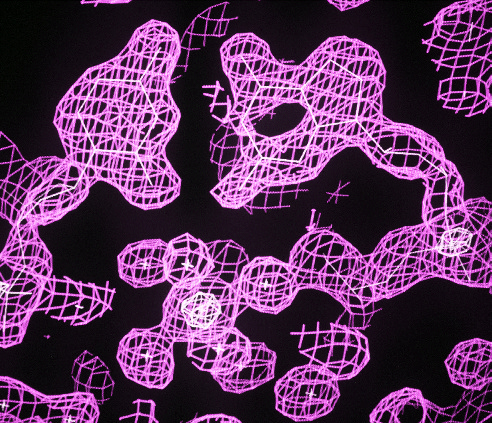
\includegraphics[width=0.5\textwidth]{Figs/xray.jpg}
\caption{Electron density map of DNA crystal \cite{Goodsell04}.}
\label{fig:xray}
\end{figure}

Besides problems with resolution, it is important to remember that the highest limitation of X-ray crystallography is simply its need of crystals, which represent one of the possible conformation, conceivably (but not necessarily) different from the one occurring in natural environment. Therefore, to overcome this issue, crystals obtained under varied conditions must be studied. This approach makes studying functional aspects of biomolecules possible.
\subsection{NMR Spectroscopy} %Subsection - 2.1.2
Another way of obtaining structural data of biomolecules is nuclear magnetic resonance (NMR) spectroscopy. It provides information about local environment of atomic nuclei. It is possible thanks to the fact, that atomic nuclei have magnetic moment, which may be aligned in a strong magnetic field. This state may be disrupted by a radio frequency pulse, which exhibits proper wavelength. What actually is measured by a spectroscopy, is the radio frequency radiation which occurs during relaxation of atomic nuclei to the basic state. It is strongly influenced by a local environment of the atom, therefore obtained data gives an information about distances between atomic nuclei and their local conformation. Usually, atomic model is developed by using a list of constraints concerning pairs of atomic neighbours and bonds between them. Its interpretation results in an ensemble of structures, which may represent all possible conformations that molecule might adopt freely in a solution or the whole range of conformations, where only one describes the actual model. In case of proteins, they differ mostly in side chains, retaining main protein chain structure.

Huge advantage of NMR technique is its applicability for molecules in a water environment, what is convenient while determining structure of biomolecules. Nevertheless, NMR spectroscopy may be used only for small proteins and nucleic acids. Even improvements in this method, such as usage of multiple radio frequency pulses which perturb multiple nuclei, enables to characterize the structure of a protein with a maximum length of 250 amino acids \cite{Goodsell04}.
 
\subsection{Electron Microscopy} %Subsection - 2.1.3
Electron microscopy methods state the approach that is the most intuitive. Nevertheless it allows to observe instead of single atoms in a molecule, only its general morphology. This issue arises from practical problems that occur while applying the technique, like imperfections of optics, problems with specimen preparations and low contrast. Therefore, the exhibited resolution is not higher than 2 nm. However, electron microscopy is often applied combined with other methods, like X-ray crystallography, NMR spectroscopy or molecular modelling. It is extremely useful not only in case of large molecules, but also to observe changes of biomolecules in different conditions. 
	\subsubsection{Transmission Electron Microscopy} %Subsection - 2.1.3.1
Transmission electron microscopy consists in illumination of a thin sample by the electron beam, whereas the microscope resolves the relative transparency of specimen regions. This method allows even to obtain a three-dimensional image by tilting the sample at a range of angles and combining resulting images (so-called electron tomography). Though, the technique is not perfect and additional proceedings are needed to improve contrast. One of them is staining the specimen with salts of heavy metals, what on the other hand may introduce artifacts. To counteract it, one may freeze the sample (cryoelectron microscopy), but it brings new problems with contrast. Thus, commonly applied approach is analysing and averaging of separate particles, which merged together give an image of whole molecule with good contrast.
	\subsubsection{Scanning Electron Microscopy} %Subsection - 2.1.3.2
Scanning electron microscopy slightly differs from its predecessor. In this approach, sample is fixed and dried and then coated with a thin metal (often golden) layer. Thereafter it is scanned with a narrow electron beam, which are scattered or emitted from a surface. This process results in a 3D image, but with relatively low resolution of 10 nm, introduced by the metal coat. Nevertheless it still may be used in research of large assemblies of biomolecules \cite{Goodsell04}.
\subsection{Atomic Force Microscopy} %Subsection - 2.1.4
The last method of determining biomolecular structures is the atomic force microscopy. It results in a topographic map of a surface of the molecule. Sample is moved under a tip both laterally and vertically (what is controlled by piezoscanners) applying a constant force on a tip. Detection of forces between specimen and cantilever is done by illuminating a laser beam on its back. Occurring reflection in different places is then caught by photo-diodes. Moreover, to reduce high shear forces that arise between tip and a sample and to prevent the latter one, the tip works in a tapping mode. Thanks to that oscillating movement, contact is shortened what minimizes shear forces. Additionally, the whole apparatus is placed in a solvent, what enables mimicking biological, natural environment and therefore give the real structure of biomolecules.

Atomic force microscopy is a really accurate tool. Its resolution depends on the sharpness of a tip, though usually is in the range between 0.1 and 10 nm. What is more, it may be applied for measuring forces between molecules or even forces that conduct protein folding \cite{Goodsell04}.
\subsection{Databases} %? %Subsection - 2.1.5
There are many kinds of bioinformatical databases, providing information about nucleotide and protein sequences, protein families, structures, their functional annotation etc. For this work the most important type constitute structural databases, therefore they are shortly described in this section.


\subsubsection{PDB}
Protein Data Bank (PDB) database was established in 1971 in USA as the tool needed for crystallographers to freely exchange protein structures between laboratories. Nowadays PDB constitutes the greatest collection of spatial structures of proteins in the world, especially since 2003, when it has been united with European Macromolecular Structure Database and PDB Japan. 

In the described database one can find structures obtained with a large variety of methods, mainly by X-ray crystallography, NMR spectroscopy and electron microscopy, which were described earlier. Before publishing of the results sent by laboratories, structure is checked for correctness and data format. Data may be presented in three kinds of files: PDB, mmCIF (macromolecular Crystallographic Information File) and PDBML (Protein Data Bank Markup Language). In the end, the structure is tagged and becomes its unique identity number. 

It is worth mentioning  the details of PDB data format, as it is mainly used by visualisation software. First of all, those files  employ so-called method of chemical rules in generating bonds between atoms. Practically, it means that there is a need of tables with types and typical lengths of bonds between certain atoms. Thanks to that, for example, if two carbon atoms are 1.5 {\AA} apart, it is assumed that they are bonded with single bond and thus the amount of information in one file is reduced. On the other hand, this solution is problematic in unusual cases, when such estimations are incorrect. What is more, data in the PDB files is divided into two groups. First one, explicit sequence, is marked with the lines with a SEQURES symbol, where one can find sequence of amino acids in certain chain of protein. However, to reconstruct the whole structure it is not enough, therefore implicit sequence is needed. In this type every single atom is represented separately with its position in Cartesian coordinate system in the space (x, y, z), its name, number in the structure, the number of the residue that atom belongs to, number of possible conformations etc. Those lines are assigned with an ATOM (usually for atoms belonging to nucleic acids or proteins) or HETATM (for small molecules) symbol \citep{Gruca10}. The whole format description and the contents guide is found on the website of Worldwide Protein Data Bank.

\subsubsection{MMDB}
Molecular Modelling Database (MMDB) which belongs to National Center for Biotechnology Information (NCBI) is strictly connected with the PDB structures, but it is extended with Entrez system, which enables the access to all biological data concerning the molecule. In this case, PDB file is translated to the ASN.1 (Abstract Syntax Notation) format, where one can additionaly find such information as unified definition of secondary structure or the spatial domain structure. In contrast to PDB files, ASN.1 contains data about every bond specifying its category (explicit bonding approach). Nevertheless it uses so-called dictionary of the residues, where atoms and bond of 20 amino acids and 8 nucleotide groups are described \citep{Gruca10}.

%********************************** %Second Section  *************************************
\section{Representation of Structures with Computer Graphics}   %Section - 2.2 
To explore and understand the working mechanisms of biomolecules, the already known structure needs to be visualized. Obviously, direct imaging in this case is impossible, as molecules are significantly smaller than the wavelength of visible light. To overcome this issue, a large variety of representations have been developed and are useful for different purposes. All of them should have two things in common: clarity - being understandable for the user and maintaining the properties of a molecule that are directly related to the nano-scale world. Here, a few most popular ones are described.

\begin{figure}[h] 
\centering    
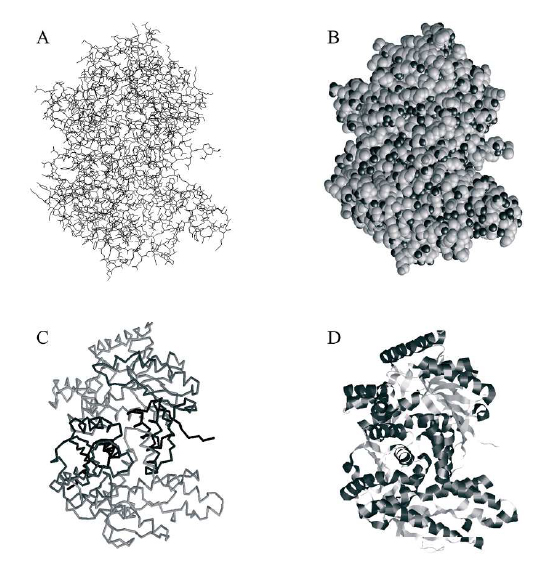
\includegraphics[width=0.8\textwidth]{Figs/visualization.jpg}
\caption{Lactate dehydrogenase presented in four ways: A- wireframe (bond diagram), B- spacefilling, C- backbone (ribbon), D- secondary structure (cartoon) diagram \cite{Gruca10}.}
\label{fig:visualization}
\end{figure}

First one, which is so-called "Ball-and-Stick" representation is the most fundamental one, presenting atoms as "balls" and bonds between them as "sticks". Although this approach is typical for education purposes, it does not provide relevant information. Most of all, it is misleading in case of the volume that molecule occupies, as the spheres are smaller than atomic radii to obtain the clearer view. Certainly, bonds presented as sticks give a comprehensive image for the user, nevertheless it is distant from the reality.  
Secondly, wireframe diagram (Figure \ref{fig:visualization} A) is simply representation of covalent bonds between atoms, presenting them as lines. It gives, similarly to "Ball-and Stick" approach, a view for the geometry of a whole molecule and finds an application in investigating linkings of proteins with cofactors or structures of active sites. On the other hand, spacefilling view (Figure \ref{fig:visualization} B) represents each atom as the relative sphere (for example Van der Waals sphere). This approach is the most relevant for size and shape representation, what is needed for visualisation of interactions between molecules. Then, ribbon diagram (known also as backbone) shows the topology of protein chain to the user and it is based on linkings between $\alpha$-carbons of each amino acid. The last representation, called "cartoon" is focused on the secondary structure of the protein, presenting $\alpha$-helices as twisted ribbons and $\beta$-sheets as arrows. Those two last examples (Figure \ref{fig:visualisation} C and D) are commonly used for topology, protein folding analysis and its comparison between different molecules \citep{Goodsell04, Gruca10}. 

Modern software used for visualisation is able to read the structural data and image it in a way that user needs. Obviously, to fulfil their task and be useful for users, such programs need to make rotation and zooming of the models possible. Moreover, additional features are helpful, such as measurements of distances and angles between atoms, identification of certain features of the structure and colouring, which significantly increases clarity of presented view. Generally user may choose from a large collection of colouring systems. In example, CPK, where each type of atom is coloured differently (carbon- grey, oxygen- red, hydrogen- white, nitrogen- blue etc.), shapely colouring, where each amino acid or nucleotide has got a different shade, chain, which, instinctively, differentiates each chain, group, where C- and N- or 3' and 5' ends are coloured differently, temperature, which helps to identify vibration degree of freedom for each atom etc \citep{Gruca10}. What is more, some of the software is not only visualisation tool and often provide a large engine for molecular modelling simulations, like program called VMD. On the Protein Data Bank Website, one can find a list of 41 programs used for biomolecular visualisations, some of them with open source or academic license.
 
%********************************** %Third Section  *************************************
\section{Virtual Reality in Visualisation of Structures}%Section - 2.3
Nowadays, a large amount of model organisms proteins have been researched and their structures are currently available in the data banks. This improvement coincides with the lastly observed computer processing power and memory growth. With addition of steady decrease of hardware prices, those occurrences create a great conditions for development of biomolecular visualisation, which leads to application of Virtual Reality for chemical and biological sciences.

\subsection{Motivation}
The most important investigation which should be done, is considering, whether engaging VE to bioinformatics is worth trying, and if so, what are the potential benefits from that solution. To answer these questions, it is convenient to describe issues that currently scientists have to deal with. First of all, for better understanding of proteins functions, their interactions and conformational changes should be known, and that is possible with the dynamically explored visualisation. Although classical approach results in still improving programs, it creates the 3D representation in the two-dimensional space, where depth perception and immersion is often not sufficient. Moreover, when several models are needed to be imaged at the same time, the view becomes unclear and structure manipulating becomes more difficult. Problem appears as well when small changes occur, such as in transient state interactions, which should be easily observable for better phenomena explanation. Furthermore, in the bioinformatics field, the human factor still plays an important role, for example in the structure interpretation and solving (often by comparative modeling) or in receptor docking simulations, when the algorithms cannot perform sufficient visual pattern recognition. Those subjects are highly important in drug design. For example, if the protein binding site is unknown, searching for possible sites need to be performed by experienced researcher and this case requires as best graphical representation of a structure as possible. Additionally, thanks to precise observations of a protein binding site, scientist may form a good hypothesis for ligand design, what is one of the most interesting tasks of molecular modelling \citep{Anderson99}. 

Those issues can be overcome or at least become easier thanks to Virtual Reality, due to its immersion effect, its intuitiveness and possibility of real-time visualisations creation. Three-dimensional image enables direct manipulation of models and interactions between them. It facilitates observation from different points, looking around and distinguishing of each structure. Although this idea does not mimic any known real surrounding, it creates an exact representation of nano-reality and enables discovering its features. Molecular modelling, molecular dynamics and bionanotechnology tools may be implemented in VR environment, creating a powerful combination that facilitates a large variety of bioinformatics tasks.  

\subsection{Examples}

The idea of combining Virtual Environment with biomolecular simulation is not new. Already described in Chapter \ref{chapter1}, \textit{GROPE} and CAVE systems were used for those purposes in 1990s. Both were applied to drug-enzyme docking procedure, while the latter was a visualisation system, which actually had its input in discovery of new molecular features. Nevertheless, it was really expensive and, what is more disturbing, it did not give the user a reference point where he or she is in the virtual world. It hinders image manipulation and gives user a feeling of disorientation \citep{Mazuryk96, Schulze11}. Then, in 2000, Abraham Anderson and Zhiping Weng created program called \textit{VRDD}, which was actually a drafting table-style projection system with additional wand with buttons, which was a program controller and remote. Additionally, the concept allowed to use a keyboard for more complex tasks. \textit{VRDD} could present different display models, enabled docking simulations, real-time calculation of binding free energies and searching for binding sites by restricting it to possible regions \citep{Anderson99}. Next, the very specific tools for VR were made, like the one designed for nucleic acids only, which can create long chains and therefore generate huge amount of data \citep{Herisson05}, or one for bionanorobotics prototyping, which main task was to invent protein-based molecular machines with usage of molecular dynamics methods \citep{Hamdi08}.

The last example constitutes \textit{Molecular Rift}, the program implemented in 2015 for \textit{Oculus Rift} by Magnus Norrby et al. What is more, it makes use of \textit{MS Kinect} gaming sensor for gesture steering, which has its equivalents in keyboard steering as well. \textit{Molecular Rift} is able to read three structure file formats: PDB, MOL2 and SDF and to perform calculations with several forcefields thanks to usage of \textit{Open Babel} chemical tool kit, make representations in different styles and colours and label specific atoms or amino acids. Additionally, the authors made user tests, which encourage to further improvements, as, despite some minor problems, the tool was rated as useful and interesting by the group of scientists \citep{Norrby15}. 

\subsection{Problems and future}

Despite all the advantages of VR application to bioinformatics, it also generates difficulties, which need to be overcome to make it a standard technology in molecular visualisation. Performance limitations constitute one of them. Complexity of the vast majority of biomolecules generates high computational cost if visualized, increasing the demand for CPU and GPU processing power of the computer. Although technological development causes new solutions that provide better efficiency of computers, the overall performance may be improved on the software site as well. In example, developers of \textit{ADN-Viewer}, program dedicated for nucleic acids imaging, implemented the idea of decrease of image quality with the distance from the user. It means, that the closest objects were represented in great details, whereas further ones- with lower accuracy. Moreover, they applied algorithm that deletes currently hidden parts of the structure from the data, what saves computational expenses \citep{Anderson99}. 

Next problem that occurs while developing for VE is the issue of navigating tools, which are necessary for the proper exploration of biological structures. In three-dimensional space it is problematic to place 2D control panel. What is more, as currently most common gear for VR is a Head-Mounted Display, which is not transparent, limitations of external input devices (mouse, keyboard, joysticks) usage occur. Nevertheless this difficulty decreases, thanks to new possibilities that appear on the market, like VR gloves, eye-tracking devices, cameras etc. However, need of such specialised equipment generates additional costs. Anyway, the rule which need to be followed is that the program should be made in a way that minimizes the possibility of user disorientation \citep{Anderson99, Norrby15}.

It is important to remember, that creating visualisation programs for VE requires cooperation of programmers and biologists, to make it as effective and useful as possible. Although there is still no software available commercially for described purposes, many papers reports new solutions in this topic, what indicates the need of visualisation improvement. Nowadays, biotechnology development and the speed of this development is strongly dependent from bioinformatics, thus one can conclude, that the potential market is relatively large. Additionally, next step in this issue for the future development is the visualisation of whole cells or even biological pathways and organelles, as Norby et al. suggest the idea of such representations, with the function of simulating and steering the biological regulation. Furthermore, it should be stressed out that scientific usefulness of VR is followed by educational one. Understanding the contents of big data largely depends on the way it is presented. Surely "gamification" and interactiveness of biochemistry could make it more attractive and assimilable for students, what may happen to be a good investment in science in the future \citep{Norrby15}.  
%makeindex <filename>.nlo -s nomencl.ist -o <filename>.nls
\nomenclature[z-mmCIF]{mmCIF}{macromolecular Crystallographic Information File}
\nomenclature[z-MMDB]{MMDB}{Molecular Modelling Database}
\nomenclature[z-NCBI]{NCBI}{National Center for Biotechnology Information}
\nomenclature[z-NMR]{NMR}{Nuclear Magnetic Resonance}
\nomenclature[z-PDB]{PDB}{Protein Data Bank}
\nomenclature[z-PDBML]{PDBML}{Protein Data Bank Markup Language}

